\documentclass[11pt,margin=1in]{scrartcl}
\input{template/structure.tex}
\usepackage{xeCJK}
\usepackage{amsmath}
\usepackage{subcaption}
\usepackage{breqn}
\usepackage{graphicx}
\setCJKmainfont{Noto Serif CJK TC}
\graphicspath{ {./img/} }
\newcommand{\vect}{\boldsymbol}
\title{
	\normalfont\normalsize
	\textsc{National Cheng Kung University}\\
	\vspace{25pt}
	\rule{\linewidth}{1pt}\\
	\vspace{20pt}
	{\huge Optimization Design Homework 3}\\
	\vspace{12pt}
	\rule{\linewidth}{2pt}\\
	\vspace{12pt}
}
\newcommand{\vect}{\boldsymbol}
\author{\Large Andr\'es ponce\
	\and 彭思安
	\and P76107116
}
\date{\normalsize\today}
\begin{document}
\maketitle
Suppose you are given this data set: $x = [0.1, 0.9, 1.9, 2.3, 
3, 4.1, 5.2, 5.9, 6.8, 8.1, 8.7, 9.2, 10.1, 12]$; $y = [20, 24, 27, 29,
32, 37.3, 36.4, 32.4, 28.5, 39, 38,43, 40, 32]$.

\section{Find (analytically) the coefficients of the best-fit linearand quadratic
regression equations. You can do it by hand or use some computer software to perform the 
calculation.}
To measure the effectiveness of our model, for the linear case we try to find the 
parameters $(a,b)$ that minimize the mean square error 
\begin{equation}
	\label{eq:mse}
	%\hat{y} = a\vect{x} + b
	\frac{1}{N}\sum_{i=1}^{N}(y_i - \hat{y}_i)^2
\end{equation}
where $\vect{y}$ is a vector containing the sample outputs, and $\hat{\vect{y}}_i$ is defined as
\begin{equation}
		\hat{y}_i = ax_i + b
	\label{eq:linear}
\end{equation}

To solve the problem analytically, we can use the formula 

\[a = (x^Tx)^{-1}x^Ty \]
which yields $a = 4.421$.
The results are shown in Figure~\ref{fig:analytical}.
\begin{figure}
	\centering
	\begin{subfigure}{0.4\textwidth}
	
		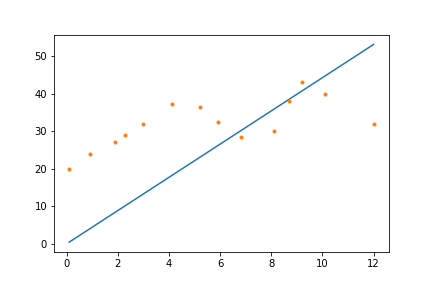
\includegraphics[scale=0.4]{p1Linear}
		\caption{Analytical linear model.}
		\label{fig:p1Linear}
	\end{subfigure}
	\hfill
	\begin{subfigure}{0.4\textwidth}
	
		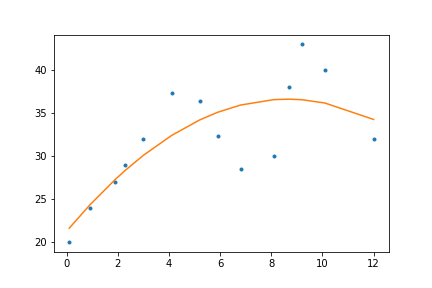
\includegraphics[scale=0.4]{p1Quad}
		\caption{Analytical quadratic model.}
		\label{fig:p1Quad}
	\end{subfigure}

	\caption{Analytical solutions to line-fitting.}
	\label{fig:analytical}
\end{figure}




Fitting a quadratic equation to the data is similar to the linear case.
The form is given by 
\begin{equation}
	\label{eq:quadratic}
	f(a, b, c) = ax^2 + bx + c
\end{equation}
and we can analytically find $(a, b, c)$ with the formulas
$$\bar{x} = \frac{1}{n}=\sum_{i=1}^{N} x_i\quad \bar{x}^2 = \sum_{i=1}^{n}x_i^2\quad\bar{y} = \frac{1}{n}\sum_{i=1}^{n}y_i$$
$$S_{xx} = \sum_{i=1}^{n}(x_i - \bar{x})^2$$
$$S_{xy} = \sum_{i=1}^{n}(x_i-\bar{x})(y_i-\bar{y})$$
$$S_{xx^2} = \sum_{i=1}^{n}(x_i - \bar{x})(x_i^2 - \bar{x}^2)$$
$$S_{x^2x^2} = \sum_{i=1}^{n}(x_i^2 - \bar{x}^2)^2$$
$$S{x^2y} = \sum_{i=1}^{n}(x_i^2-\bar{x}^2)(y_i-\bar{y})$$

The formulas give $f(x) = -.206x^2 + 3.567x + 21.262$ as our parabola, also shown in Figure~\ref{fig:analytical}.
\section{Find the best fit coefficients of the linear and quadratic 
regression equations numerically. First, use the Fletcher-Reeves 
conjugate gradient method. Then use one of the methods involving Newton's method or one of the 
quasi-Newton methods (DFP or BFGS).}

We optimize the Equation~\ref{eq:linear} and Equation~\ref{eq:quadratic} first by using Fletcher-Reeves, then by 
using the BFGS algorithms.
The code implementations can be found in the attached jupyter notebook, and the graphs for our approximations using
these algorithms is shown in Figure~\ref{fig:p3a} and Figure~\ref{fig:p3b}.
The quadratic approximation using Fletcher-Reeves does not appear like the estimates in other problems, maybe this 
an implementation error. 
The other implementations agree with our analytical estimates.

\begin{figure}
	\centering
	\begin{subfigure}{0.4\textwidth}
			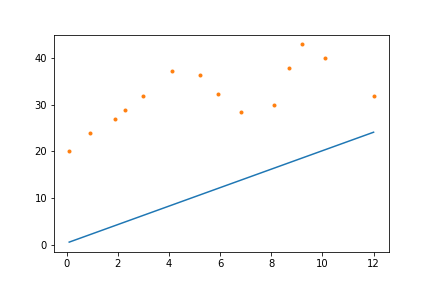
\includegraphics[scale=0.5]{FRLinear}
	\end{subfigure}
	\begin{subfigure}{0.4\textwidth}
			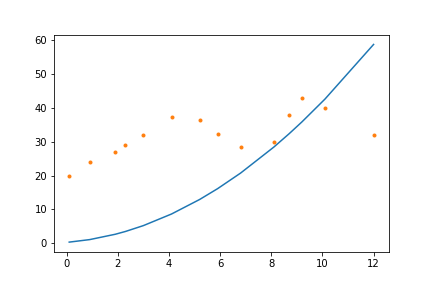
\includegraphics[scale=0.5]{FRQuad}
	\end{subfigure}
	\caption{Linear and quadratic regression using Fletcher-Reeves.}
	\label{fig:p3a}
\end{figure}

\begin{figure}
	\centering
	\begin{subfigure}{0.4\textwidth}
			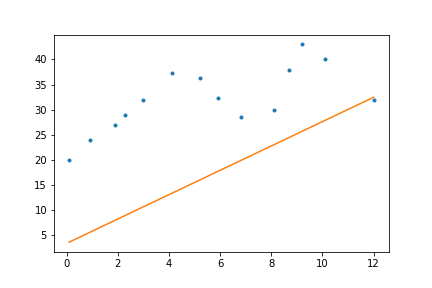
\includegraphics[scale=0.5]{BFGSLinear}
	\end{subfigure}
	\begin{subfigure}{0.4\textwidth}
			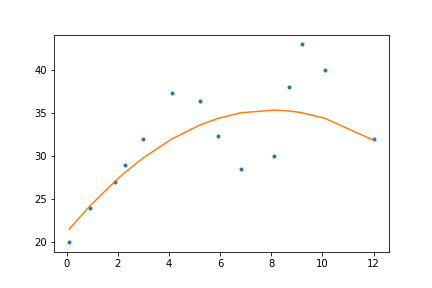
\includegraphics[scale=0.5]{BFGSQuad}
	\end{subfigure}
	\caption{Linear and quadratic regression using BFGS quasi-Newton method.}
	\label{fig:p3b}
\end{figure}

\section{With polynomial regression, decide the order of the polynomial
which reasonably fits the data without making the order too high.}
\begin{figure}
	\centering

	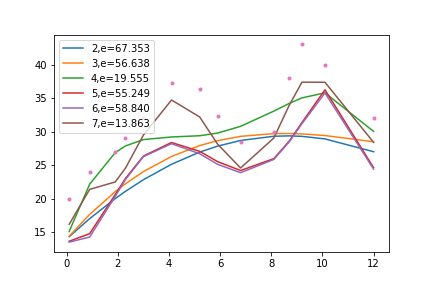
\includegraphics[scale=0.5]{p3}
	\caption{Estimation of input data with higher order polynomials.}
	\label{fig:orders}
\end{figure}

To obtain the $n$-th order polynomial model, we can use \texttt{numpy}'s \texttt{polyfit} method, which takes 
$x, y$, and order $n$ as input.
The models using different orders and errors $e$ are shown in Figure~\ref{fig:orders}.
Similar to our quadratic and linear models, $n=3$ fails to capture the wave-like pattern of the input.
The fourth order polynomial starts to capture the curves, but when $n=5$ or $n=6$ we see the best balance
of learning the input pattern and generalization ability.
These two orders similarly capture the curves of our model without capturing too much of the noise.
For $n=7$, although the error is still lower than the other orders, the line starts getting too close to the 
input, which might indicate overfitting and poor performance across other inputs.

\section{Use your creativity to construct the regression model (i.e. combining polynomials, $\sin(x)$, $\cos(x)$, $e$ and/or $\log(x)$ functions) which 
best fits the data. Also, describe your reasons for choosing certain functions in your models.}
When creating our model, we are looking to ensure some characteristics.
First, the input pattern has some wave-like pattern, similar to a periodic function such as $\sin(x)$.
Second, the input points also seem to curve inward; they are not perfectly linear.
The $\sin$ and $\log$ functions seem to match these requirements quite well.
We can write our objective function as 
\begin{equation}
	f(x) = c_1x\log(1 + x + c_2\sin(x))
\end{equation}
where we want to find the $c_1, c_2$ that minimizes the error of this function.
The gradient of this function is 
\begin{equation}
	\nabla f =
	\begin{bmatrix}
		\frac{\partial f}{\partial a} \\
		\frac{\partial f}{\partial b}	
	\end{bmatrix}
	=
	\begin{bmatrix}
			x\log(1 + x + b\sin(x))	 \\
			\frac{ax\sin(x)}{b\sin(x) + x}
	\end{bmatrix}
\end{equation}

Using steepest descent with the learning rate $\eta = 0.001$, we run our model by moving in the direction of $-\eta\nabla f$ for twenty thousand 
iterations.
The result is shown in Figure ~\ref{fig:p4OwnModel}.
While the figure also has some slight curves, with our training it does not match the ability of some higher order polynomials.
This could be due to errors in the training procedure, with adjustments to the parameters it might be possible to better fit the data
with this function.
\begin{figure}
	\centering
	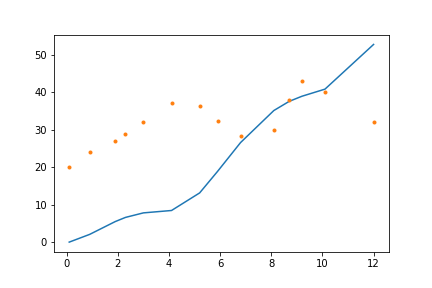
\includegraphics[scale=0.5]{p4OwnModel}
	\caption{Our own approximation using $ax\log(1 + x + b\sin(x))$.}
	\label{fig:p4OwnModel}
\end{figure}

\end{document}

